\documentclass[conference]{IEEEtran}
\IEEEoverridecommandlockouts
% The preceding line is only needed to identify funding in the first footnote. If that is unneeded, please comment it out.
\usepackage{cite}
\usepackage{amsmath,amssymb,amsfonts}
\usepackage{algorithmic}
\usepackage{graphicx}
\usepackage{textcomp}
\usepackage{xcolor}
\usepackage{caption}
\usepackage[ngerman]{babel}
\usepackage{svg}
\usepackage{float}

\def\BibTeX{{\rm B\kern-.05em{\sc i\kern-.025em b}\kern-.08em
    T\kern-.1667em\lower.7ex\hbox{E}\kern-.125emX}}
\begin{document}

\title{Entwurf eines Rettungsroboters für Waldbrandszenarien\\
{\footnotesize \textsuperscript{*}Projekt Angewandte Elektrotechnik Gruppe 1}

}

\author{\IEEEauthorblockN{Jonas Gerken}
\IEEEauthorblockA{\textit{Hochschule Hamm-Lippstadt} \\
Lippstadt, Deutschland \\
jonas.gerken@stud.hshl.de}
\and
\IEEEauthorblockN{Niklas Heiber}
\IEEEauthorblockA{\textit{Hochschule Hamm-Lippstadt} \\
Lippstadt, Deutschland \\
niklas.heiber@stud.hshl.de}
\and
\IEEEauthorblockN{Michael Jathe}
\IEEEauthorblockA{\textit{Hochschule Hamm-Lippstadt} \\
Lippstadt, Deutschland \\
michael.jathe@stud.hshl.de}
\and
\IEEEauthorblockN{Benedikt Lipinski}
\IEEEauthorblockA{\textit{Hochschule Hamm-Lippstadt} \\
Lippstadt, Deutschland \\
benedikt.lipinski@stud.hshl.de}

}

\maketitle

\begin{abstract}
This document is a model and instructions for \LaTeX.
This and the IEEEtran.cls file define the components of your paper [title, text, heads, etc.]. *CRITICAL: Do Not Use Symbols, Special Characters, Footnotes, 
or Math in Paper Title or Abstract.
\end{abstract}

\begin{IEEEkeywords}
component, formatting, style, styling, insert
\end{IEEEkeywords}

 

\section{Systemmodellierung}
\subsection{Kontextdiagramm}
-MJ-


Zu Beginn des Systementwurfs wurde ein Kontextdiagramm erstellt( siehe Abb. \ref{fig:context}). Das Kontextdiagramm dient zur Modellierung der Systemumgebung bildet die Schnittstellen zur Umwelt ab. So soll der Rettungsroboter z.B. eine Gegensprechanlage besitzen, um eine verbale Kommunikation zwischen dem Rettungsdienst und der zu rettenden Person zu ermöglichen. Außerdem wurden im Kontextdiagramm noch weitere Anforderungen spezifiziert. So soll die Hinderniserkennung mit Ultraschallsensoren umgesetzt werden.

\begin{figure}[h]
    \centering
    \captionsetup{width=.9\linewidth}
    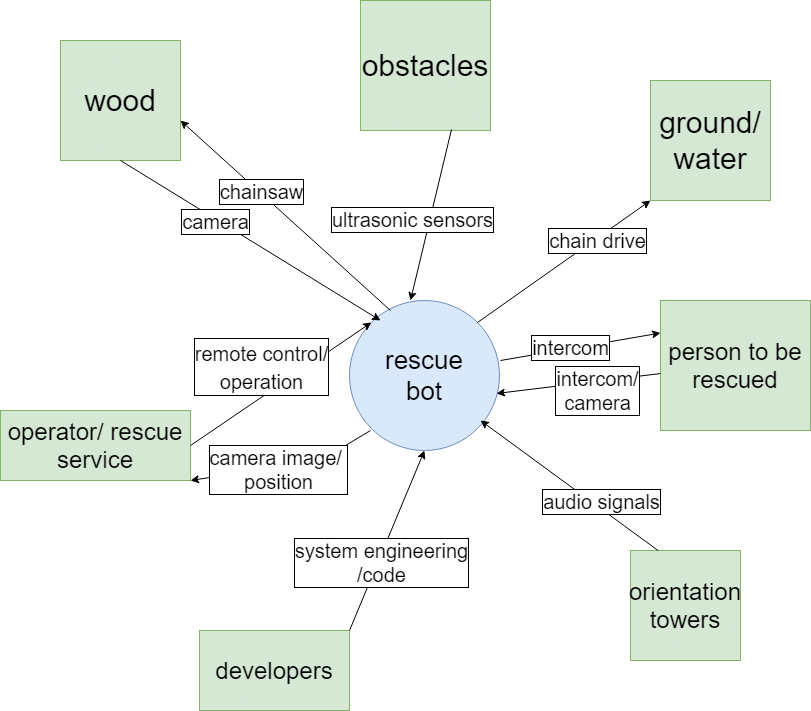
\includegraphics[width=1\linewidth]{contex_diagram.png}
    \caption{Kontextdiagramm}
    \label{fig:context}
\end{figure}

\section{3D Modell}
\begin{figure}[h]
    \centering
    \captionsetup{width=.9\linewidth}
    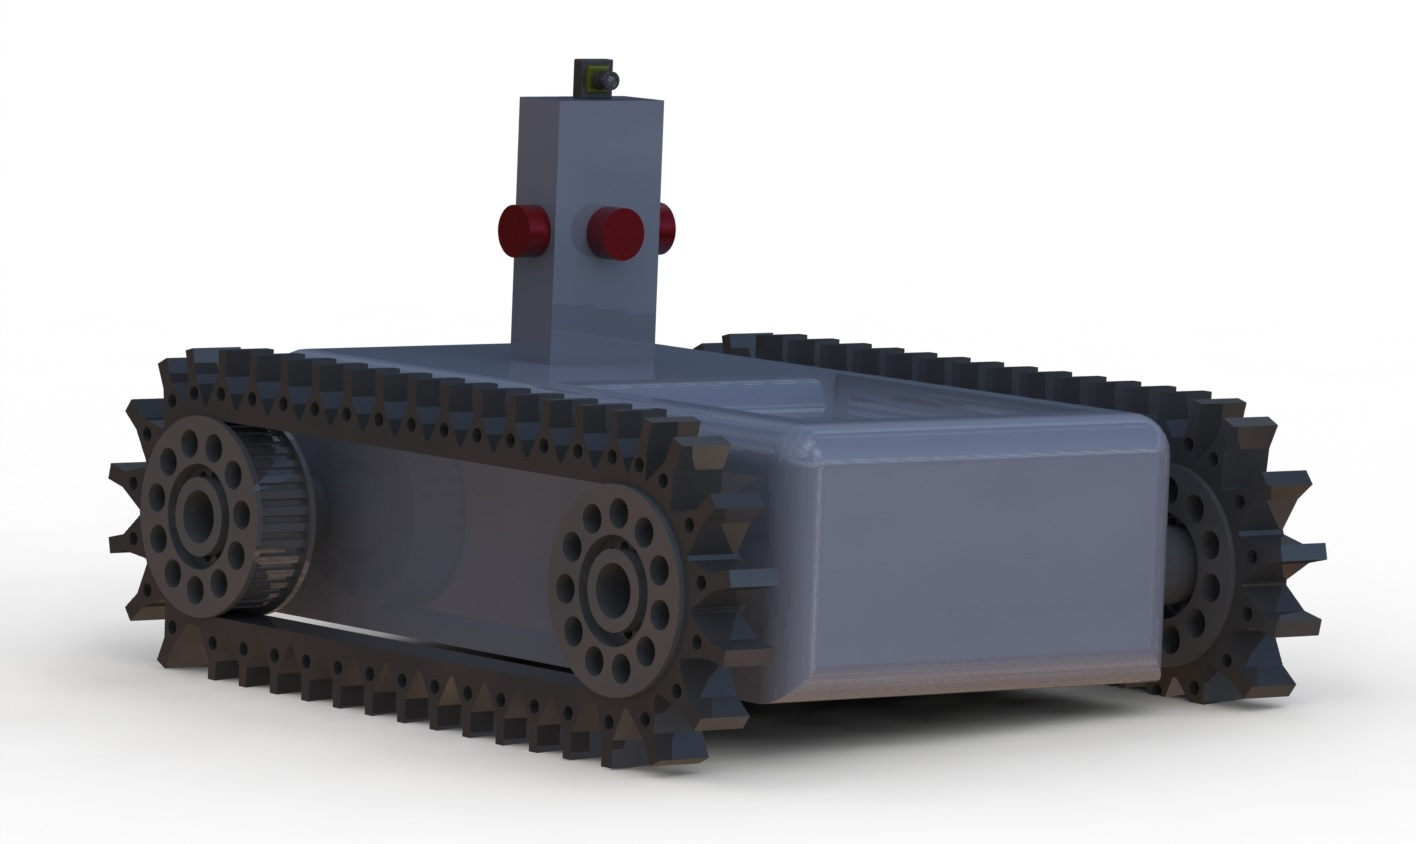
\includegraphics[width=1\linewidth]{v2_rendering.JPG}
    \caption{Erster Prototyp}
    \label{fig:prot}
\end{figure}

Das 3D-Modell des Rettungsroboters wurde mit der Software SolidWorks erstellt. Die Abbildung \ref{fig:prot} zeigt den ersten Prototyp. Hier wurden schon der Kettenantrieb und eine Ablagefläche für ein Erste-Hilfe-Kit umgesetzt. Weiter wurde auf dem Robotor ein Turm platziert, um dort 4 Sensroen für die Orientierung anzubringen. Oben auf dem Turm befindet sich eine Kamera.\\


\begin{figure}[h]
    \centering
    \captionsetup{width=.9\linewidth}
    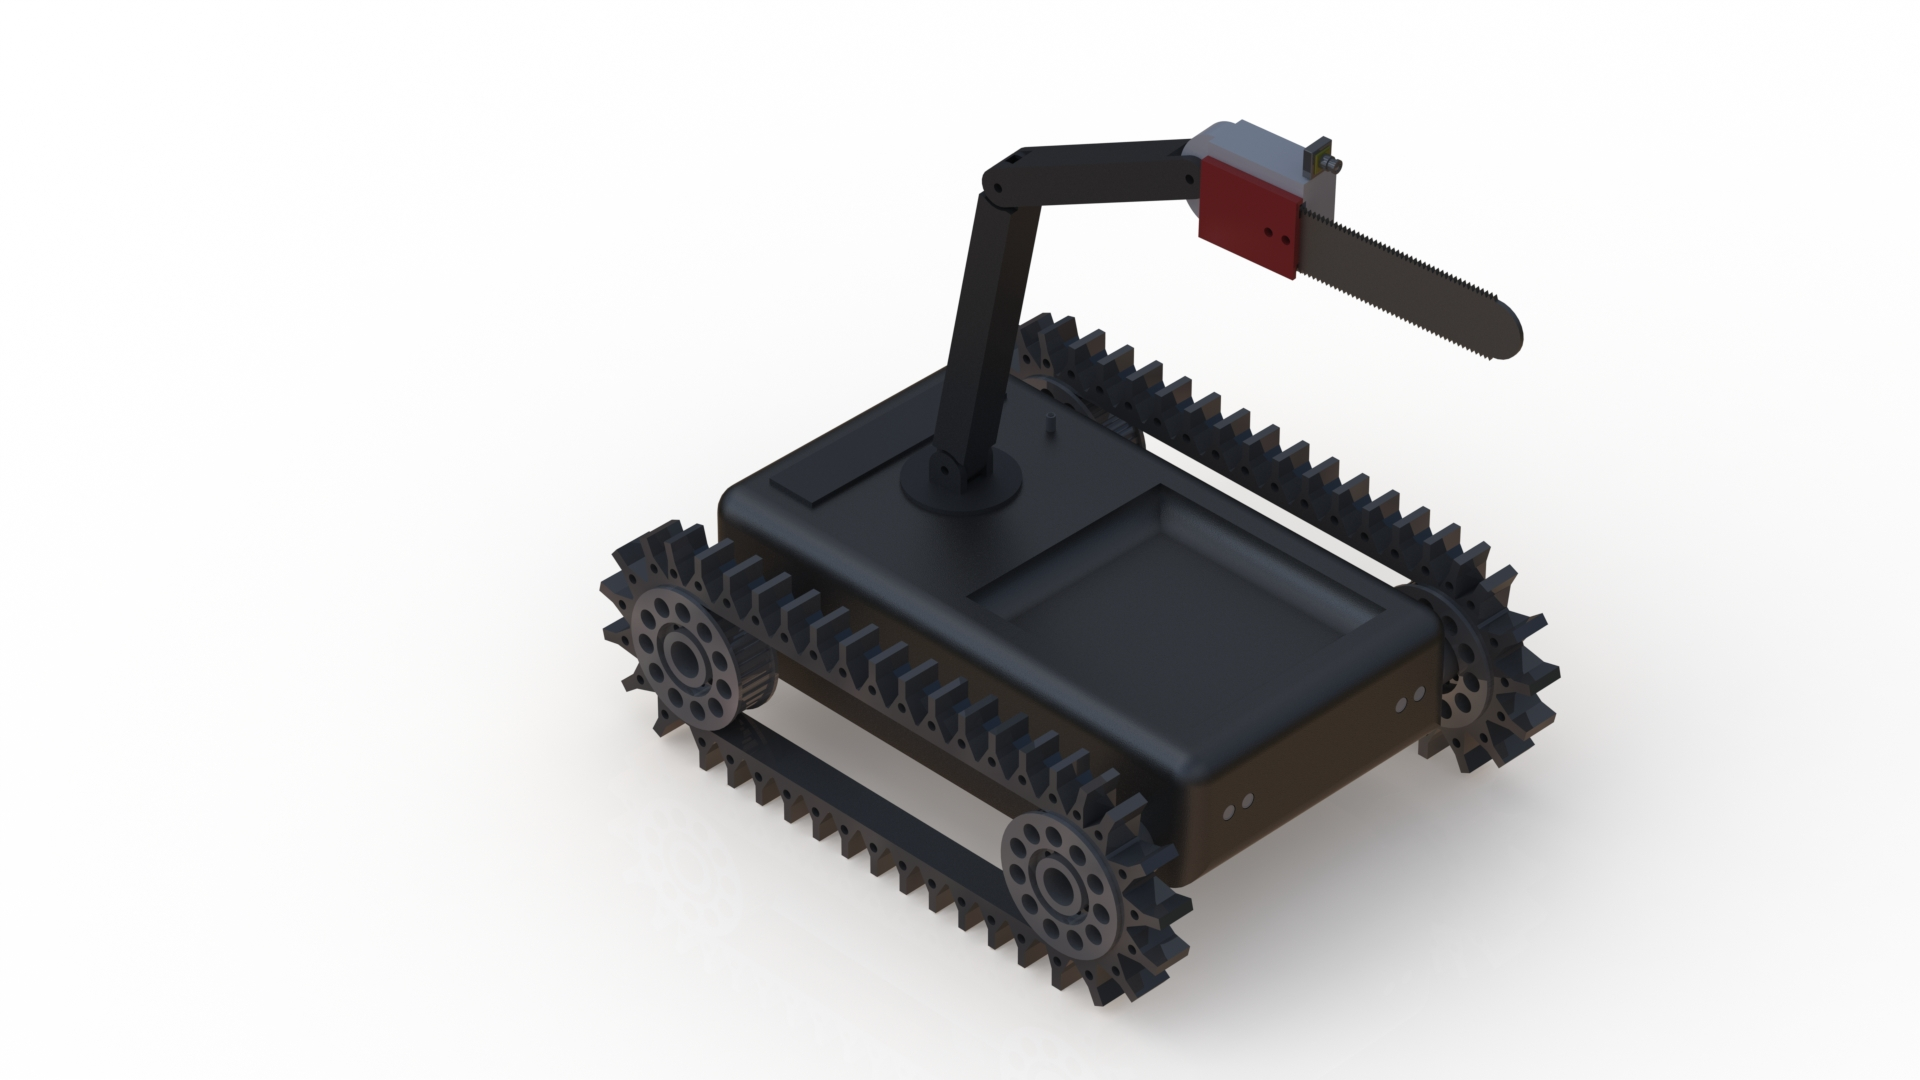
\includegraphics[width=1\linewidth]{bot_rendering_v4.JPG}
    \caption{Zweite Version den Roboters}
    \label{fig:second}
\end{figure}

Für die zweite Version des Prototyps wurde zunächst der Körper des Bots angepasst. Für eine Verbesserung des Strömungsverhaltens und einer Erhöhung des Böschungswinkels wurde der Körper an der vorderen unteren Kante mit einer sehr Flachen Fase versehen.

Im nächsten Schritt wurde der unbewegliche Turm durch einen Roboterarm mit 3 Gelenken und einer Drehscheibe ersetzt (Abb. \ref{fig:second}). Am Ende des Arms wurde eine Kettensäge angebracht. Die Kamera wurde auf der Säge angebracht, um so die Säge immer im Blick zu haben.

Weiter wurden noch ein austauschbarer Akku, ein omnidirektionales Mikrofon und Ultraschallsensoren in den Prototyp intgeriert.
\begin{figure}[h]
    \centering
    \captionsetup{width=.9\linewidth}
    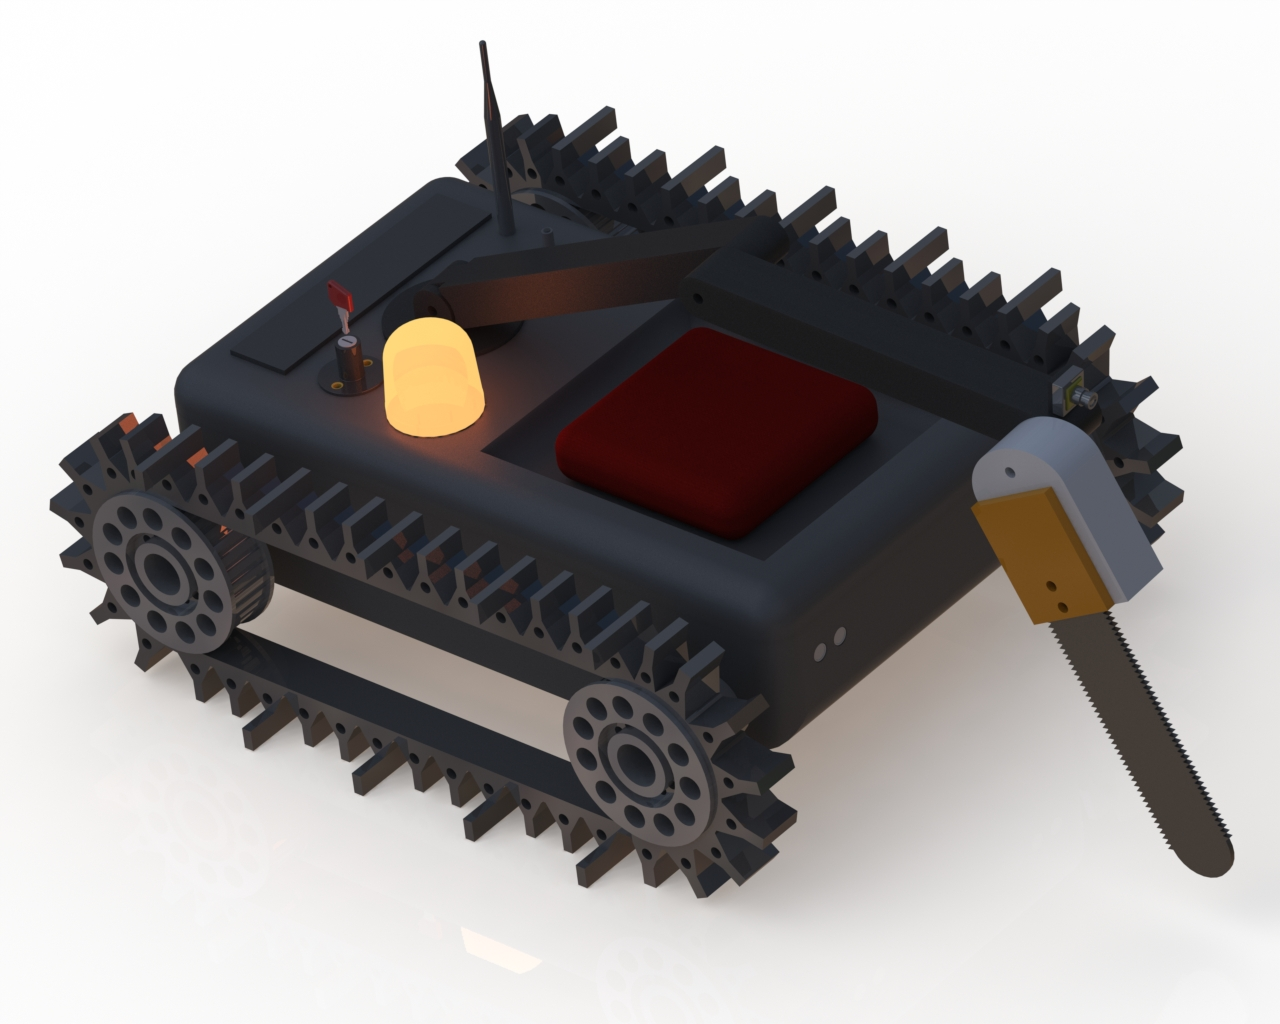
\includegraphics[width=1\linewidth]{trimetrisch_vorne_rechts_oben.JPG}
    \caption{Außenansicht des Roboters}
    \label{fig:final}
\end{figure}
\begin{figure}[h]
    \centering
    \captionsetup{width=.9\linewidth}
    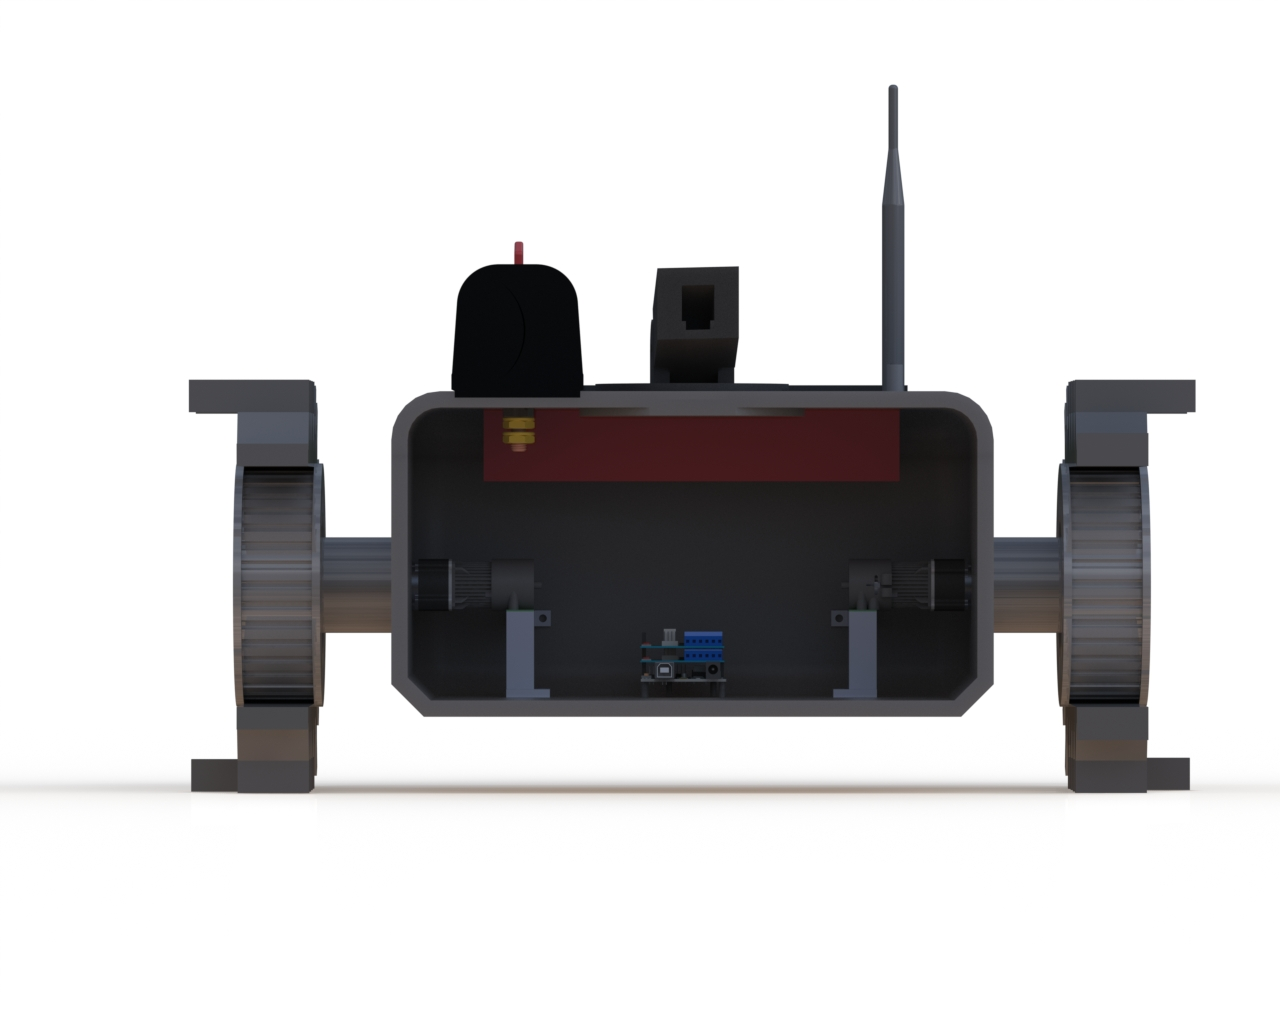
\includegraphics[width=1\linewidth]{schnitt_front.JPG}
    \caption{Schnittansicht von vorne}
    \label{fig:front}
\end{figure}
\begin{figure}[h]
    \centering
    \captionsetup{width=.9\linewidth}
    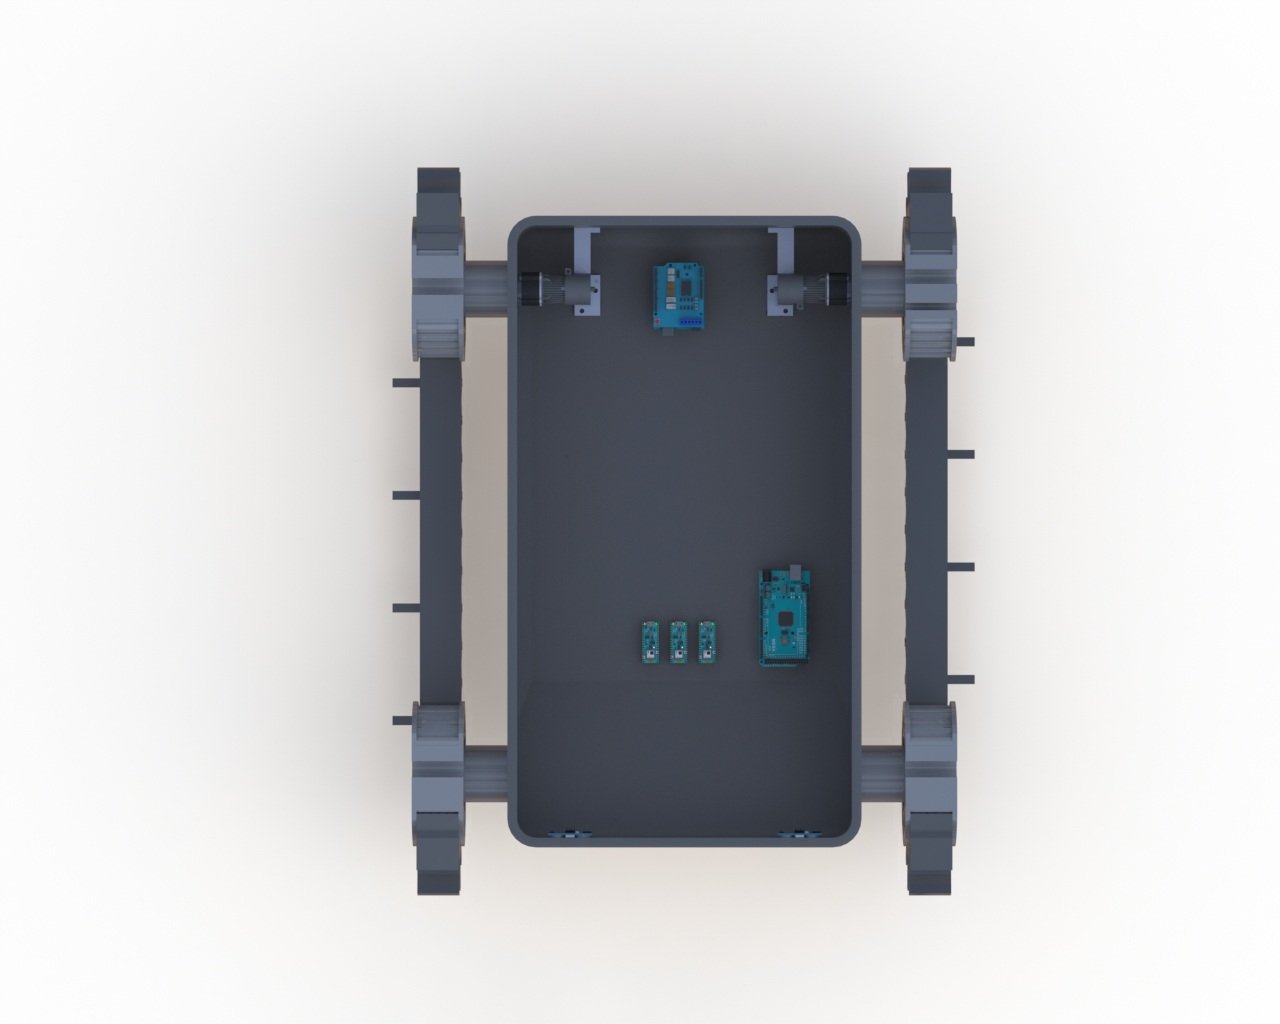
\includegraphics[width=1\linewidth]{schnitt_top.JPG}
    \caption{Schnittansicht von oben}
    \label{fig:top}
\end{figure}
\begin{figure}[h]
    \centering
    \captionsetup{width=.9\linewidth}
    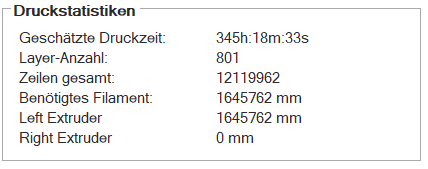
\includegraphics[width=1\linewidth]{print-statistic.PNG}
    \caption{Druckstatistiken}
    \label{fig:print_stats}
\end{figure}
\begin{figure}[h]
    \centering
    \captionsetup{width=.9\linewidth}
    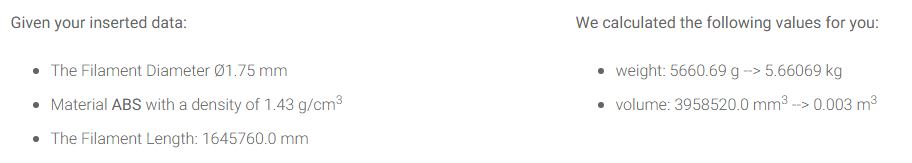
\includegraphics[width=1\linewidth]{filament_weight.PNG}
    \caption{Erechnetes Filamentgewicht}
    \label{fig:filament_weight}
\end{figure}
\end{document}
